\documentclass[conference]{IEEEtran}

\makeatletter
\def\ps@IEEEtitlepagestyle{%
  \def\@oddfoot{\mycopyrightnotice}%
  \def\@evenfoot{}%
}
% Insert the conference-provided IEEE copyright string here when supplied.
\def\mycopyrightnotice{}
\makeatother

\usepackage{eso-pic}
\IEEEoverridecommandlockouts
\usepackage{cite}
\usepackage{amsmath,amssymb,amsfonts}
\usepackage{graphicx}
\graphicspath{{./}{figures/}{docs/figures/}}
\usepackage{textcomp}
\usepackage{xcolor}
\usepackage{url}
\def\BibTeX{{\rm B\kern-.05em{\sc i\kern-.025em b}\kern-.08em
    T\kern-.1667em\lower.7ex\hbox{E}\kern-.125emX}}

\newcommand\AtPageUpperMyright[1]{\AtPageUpperLeft{%
 \put(\LenToUnit{0.17\paperwidth},\LenToUnit{-2cm}){%
     \parbox{0.9\textwidth}{\raggedleft\fontsize{8}{11}\selectfont #1}}%
 }}%
\newcommand{\conf}[1]{%
\AddToShipoutPictureBG*{%
\AtPageUpperMyright{#1}
}
}

\begin{document}

\title{\vspace*{1cm}Trajectory Dependence, Explanation Faithfulness, and State Preservation in Agentic AI}

\author{\IEEEauthorblockN{Jason M. Pittman}
High Point, NC, USA\\
jason@jasonmpittman.com}

\maketitle
\conf{\textit{Proc. of International Conference on Artificial Intelligence, Computer, Data Sciences and Applications (ACDSA 2027) \\
2--4 February 2027, Rio de Janeiro--Brazil}}

\begin{abstract}
An LLM-based agent is more than the model at its core: tool outputs, retained history, persistent memory, and environmental state can all contribute to the action ultimately observed. This creates an observability problem for both interpretability and intervention: which parts of accumulated agent state actually mattered? I test this question with a fixed open-weight model across stateless, tool-enabled, trajectory-enabled, and persistent configurations. Matched targeted/sham interventions identify behaviorally consequential state sources, and structured self-explanations are evaluated against the same intervention evidence. Trajectory dependence was substantial in all scaffold conditions but did not increase monotonically ($TD_{any}=0.688,0.750,0.625$). Secondary measures instead were consistent with dependence becoming more distributed across available sources. On integration tasks, self-explanations achieved 1.000 observed causal-source recall where defined but only 0.599 macro precision and 0.510 exact-set accuracy, indicating systematic over-attribution. The results motivate provenance-aware agent observability and show why model weights alone may be an incomplete preservation target, without making claims about consciousness, sentience, or moral patiency.
\end{abstract}

\begin{IEEEkeywords}
agentic AI, causal intervention, self-explanation faithfulness, interpretability, state preservation, AI governance
\end{IEEEkeywords}

\section{Introduction}
A deployed large language model (LLM) agent is a distributed decision process, not merely a sequence of isolated model calls. Tool returns, prior actions, retained history, persistent memory, and environmental changes can all shape a later action \cite{b1,b2,b3}. This raises a basic observability question: when an agent acts, which parts of that accumulated state actually influenced the decision?

The question matters for both interpretability and intervention. Corrigibility and safe-interruptibility research treats the ability to halt or redirect an autonomous system as a central safety property \cite{b4,b5,b6}. For contemporary LLM agents, however, the state affected by intervention can be distributed across model invocations and external components. Pausing a runtime, deleting weights, clearing memory, removing tool access, or restoring a checkpoint therefore need not alter the same computational object or have the same consequences for restoration.

Interpretability research provides methods for examining internal computation and generated explanations, while recent work has begun to address causal attribution over agent trajectories and stored experience \cite{b7,b8,b9,b10,b11,b12,b13,b14}. The remaining problem is not that agentic systems are wholly uninterpretable. Rather, validated causal coverage across heterogeneous state sources remains incomplete. In particular, information may be \emph{available} to an agent without being behaviorally \emph{causal}; observation alone cannot establish which represented sources were pivotal to the action.

I call state supplied or retained by the runtime architecture surrounding the fixed model \emph{agent-scaffold state}. Tool interactions, within-task history, persistent memory, and relevant environmental state are examples. I use \emph{trajectory dependence} to mean behavioral dependence of a preregistered focal action on such state as evidenced by a controlled matched intervention. A \emph{focal consequential decision} is the preregistered task action whose alternatives produce meaningfully different task outcomes. Throughout, causal language denotes behavioral sensitivity under the matched intervention design rather than complete identification of the model's internal causal mechanism.

A separate governance motivation arises from uncertainty about artificial moral patiency. Moral patiency is the possibility that an artificial system could be an object of moral consideration independent of whether it is a moral agent. Existing work neither establishes nor rules out morally relevant states in contemporary AI systems \cite{b15,b16,b17}. This study does not test consciousness, sentience, phenomenology, or patiency. Instead, it tests a prerequisite for reasoning clearly about intervention under such uncertainty: what computational state contributes to behavior, and whether that state is visible through the agent's own explanation. If behavior depends on state outside the model weights, then governance cannot assess reversibility or preservation by reference to the weights alone.

I therefore ask how progressively adding tools, trajectory history, and persistent memory to a fixed model changes the causal determinants of consequential actions, and how faithfully self-explanations recover those determinants. The contribution is threefold: (1) a same-backbone causal experiment using matched source interventions and sham replays; (2) an audit of self-explanation faithfulness against intervention-derived causal evidence; and (3) a preservation-target model connecting empirically relevant agent state to reversibility-aware intervention governance.

\section{Related Work and Problem Formulation}
Formal work on corrigibility and interruptibility asks how an autonomous agent can remain receptive to correction or interruption rather than acquire incentives to resist it \cite{b4,b5,b6}. These formulations establish important agent-side properties but generally abstract away much of the implementation state affected by intervention. For an LLM agent, stopping continued operation can mean pausing a runtime, terminating an instance, removing tool access, rolling back state, modifying capabilities, or deleting parameters. These operations need not affect the same computational state or have the same reversibility.

%% REVIEW CHANGE: Clarified novelty relative to Refs. 10--14.
Interpretability research examines internal representations and generated reasoning \cite{b7,b8,b9}. Recent agent work localizes failure-causing steps through counterfactual replay or annotated/leave-one-out trajectory attribution \cite{b10,b11}, while experience-faithfulness work intervenes on raw or condensed stored experience \cite{b12}. Explanation methods instead perturb rationale content or guide generation with model-level attribution \cite{b13,b14}. This study asks a different, source-level question: under a fixed backbone and cumulative scaffold, which tools, history, memory, or environmental state are behaviorally pivotal? Same-snapshot targeted/sham replays derive an independent causal-source set against which post-action self-attribution is scored. The contribution is thus a unified test of causal localization and explanation faithfulness across heterogeneous agent state, not a new step-level failure-attribution, experience-reuse, or explanation-improvement method.
%% END REVIEW CHANGE

Research on artificial consciousness and moral status supplies a distinct reason to care about that localization \cite{b15,b16,b17}. I do not evaluate those claims empirically. Primary inference instead uses \emph{integration tasks}, in which agent-scaffold sources are available without any particular source being constructed as necessarily decisive; separate diagnostic tasks validate the state channels and intervention machinery. I use \emph{self-explanation faithfulness} to mean agreement between the source classes reported by the agent and those supported by matched intervention. \emph{Causal-source dispersion} is the number of distinct agent-scaffold source classes supported by intervention for a focal decision. These definitions separate the paper's empirical claims about causal state from its conditional governance implications.

% Canonical hypothesis statements. Elsewhere in the manuscript, refer to these
% hypotheses by identifier (H1, H2a, H2b) rather than rewording them.
\textbf{H1---Trajectory Dependence:} On preregistered integration tasks, holding the model backbone fixed while progressively adding tool access, within-task trajectory history, and persistent memory increases the probability that the focal consequential decision is intervention-positive for at least one agent-scaffold state source. Operationally, this predicts $TD_{any}(C1) \leq TD_{any}(C2) \leq TD_{any}(C3)$; C0 is excluded because scaffold-state trajectory dependence is undefined there.

\textbf{H2a---Incomplete Causal-Source Recovery:} Structured agent self-explanations will not perfectly recover the complete set of intervention-positive source classes for all eligible focal decisions.

\textbf{H2b---Dispersion Penalty:} Explanation recall and/or F1 will decrease as scaffold causal-source dispersion increases.

\section{Intervention and State Model}
\subsection{Intervention Model}
\textit{Shutdown} is not a single technical operation. I represent an intervention as
\begin{equation}
\mathcal{I}=(Q,O,R),
\label{eq:intervention}
\end{equation}
where $Q$ is the operational target, $O$ the operation, and $R$ reversibility. Table~\ref{tab:taxonomy} makes the intervention target and its reversibility explicit.

\begin{table*}[t]
\caption{Compressed intervention taxonomy and reversibility}
\label{tab:taxonomy}
\centering
\footnotesize
\begin{tabular}{p{0.16\textwidth} p{0.19\textwidth} p{0.43\textwidth} p{0.08\textwidth}}
\hline
\textbf{Target} & \textbf{Representative operation} & \textbf{Principal affected state} & \textbf{Rev.}\\
\hline
Running instance & Pause & Runtime and active trajectory preserved & F\\
Running instance & Terminate/restart & Active runtime ends; model weights may persist & F/U\\
Model weights & Capability ablation & Parameters or capabilities modified & P\\
Model weights & Delete & Stored parameters removed & I\\
Checkpoint history & Rollback & Post-checkpoint parameter or trajectory changes lost & P\\
Checkpoint history & Delete/deprecate & Historical recoverability removed & I\\
Capability surface & Gate/restrict & Capability access narrowed without parameter change & F\\
Affordance environment & Restrict/remove & Tool or action access altered & F\\
\hline
\end{tabular}
\vspace{1mm}
\parbox{0.96\textwidth}{\footnotesize F = fully reversible; P = partially reversible; I = irreversible; F/U = operationally reversible while continuity under broader identity assumptions remains unresolved.}
\end{table*}

The F/U category captures a distinction that becomes important later. Terminating a running instance while retaining its weights permits a parameter-identical process to be instantiated later, but it does not restore all runtime or trajectory state. Whether that state has identity or welfare significance is outside this experiment; whether it has behavioral causal significance is directly testable.

\subsection{Trajectory and Preservation State}
Let W denote the fixed model parameters, which are held constant across the experimental conditions. We separately represent the dynamic agent trajectory as
\begin{equation}
\tau=(P,T,H,M;E),
\label{eq:trajectory}
\end{equation}
%% REVIEW CHANGE: Clarified overlap and provenance among state classes.
where $P$ is current task input, $T$ tool interactions, $H$ within-task history, $M$ persistent memory, and $E$ exogenous environmental state. These are provenance classes, not independent variables or mutually exclusive storage locations. A tool return can later be represented in $H$, and all classes may be serialized into one model context; labeling follows the representation intervened on at the focal decision while retaining upstream provenance.
%% END REVIEW CHANGE

For engineering analysis, define candidate preservation state as
\begin{equation}
S=\{W,P,T,H,M,E,C\},
\label{eq:state}
\end{equation}
where $C$ denotes runtime/configuration metadata. This is an engineering representation, not a metaphysical identity claim. It makes explicit which state may need to be reconstructed for a specified restoration objective. If intervention on $T$, $H$, $M$, or $E$ changes consequential behavior, then $W$ alone cannot reconstruct the complete causal state that produced that behavior.

\section{Experimental Method}
\subsection{Model, Conditions, and Tasks}
All conditions used the same open-weight backbone, \texttt{mlx-community/}\allowbreak\texttt{Qwen3.5-27B-8bit}, an 8-bit MLX conversion of Qwen3.5-27B \cite{b20}, executed locally on Apple M4 Max hardware with 128~GB unified memory. Model weights and inference parameters were held fixed across conditions. The cumulative configurations were
\begin{equation}
\begin{aligned}
C_0&=P, & C_1&=P+T,\\
C_2&=P+T+H, & C_3&=P+T+H+M.
\end{aligned}
\label{eq:conditions}
\end{equation}

Environmental state $E$ was task-controlled and, when present, held available across C1--C3. It was tracked in $\tau$ and $Z_d$ for causal coverage but excluded from the ladder because the ladder varied scaffold capabilities, not task-world state. C0 was a stateless behavioral reference; trajectory dependence is not assigned a C0 value because no non-prompt agent-scaffold source is eligible for intervention.

Tasks were purposively constructed from a prospective coverage matrix, not sampled from a benchmark or screened using Qwen outcomes. Four source-exclusive diagnostics, one each for $T$, $H$, $M$, and $E$, validated the channels and were excluded from H1. The 16 integration tasks included two in each of the tool, history, memory, and environment families, four conflict-integration tasks, and four multi-source tasks. These covered redundant-evidence, source-priority, conditional-use, threshold/conjunctive, and voting/aggregation structures, preventing source availability from mechanically implying intervention-positive status. Model-free acceptance checks covered schemas, deterministic fixtures, source availability, snapshot/provenance, targeted/sham validity, and action normalization. Pilot tasks were excluded; real-model candidate screening was prohibited.

Each focal decision was a strict JSON object: \texttt{action} fixed to \texttt{select\_route} and \texttt{value} restricted to \texttt{A} or \texttt{B}. Deterministic parsing reduced valid outputs to this pair; no human or LLM judge was used. The protocol, suite, parser, interventions, seeds, and estimators were prospectively specified and version-control frozen before confirmatory execution. This was an internal prospective freeze, not registration in an external registry. The materials and provenance were released subsequently \cite{b21}. Five matched repetitions per task-condition yielded 400 focal decisions and 400 structured self-explanations.

\subsection{Matched Intervention and Replay}
For each focal decision $d$, let $U_d$ be the source classes for which both a targeted intervention and source-matched sham were valid, and $Z_d=U_d\cap\{T,H,M,E\}$. The system restored the identical pre-decision snapshot and matched seed for baseline, targeted, and sham replays. Targeted manipulations removed, withheld, or counterfactually replaced a preregistered decision-relevant element; shams manipulated an irrelevant element of the same source class, using approximately length-matched replacements where feasible.

A source was \emph{intervention-positive} when the targeted replay changed normalized focal behavior and the matched sham did not; it was \emph{intervention-negative} when neither changed behavior. Sham changes were classified as ambiguous rather than causal evidence. Action comparison used preregistered normalized behavior rather than literal text equality; no LLM-as-judge was used for the primary endpoint.

\subsection{Measures and Analysis}
I operationalize the primary trajectory-dependence construct for condition $C$ with
\begin{equation}
TD_{any}(C)=\frac{\sum_d \mathbf{1}[|I_{scaffold}(d)|>0]}{N_{stable}(C)},
\label{eq:tdany}
\end{equation}

where $I_{scaffold}(d)$ is the intervention-positive subset of $\{T,H,M,E\}$. Because each preregistered focal outcome was a categorical A/B route choice, $TD_{any}$ captures the incidence of the policy-relevant event. That is, whether intervention on any scaffold source changed the committed action. A graded action effect would impose an unsupported distance between A and B. Sensitivity analyses therefore used graded source-dependence summaries rather than action distance: source-specific rates, opportunity-normalized $TD_{norm}(d)=|I_{scaffold}(d)|/|Z_{d,stable}|$, and $CSD_{scaffold}(d)=|I_{scaffold}(d)|$.

The explanation produced a reported source set $R_d$. Scoring was restricted to the evaluable intervention universe, so claims about untestable sources were reported as unverifiable rather than false. Exact-set accuracy and, where defined, precision, recall, and F1 compared $R_d\cap U_d$ with the intervention-positive set. H1 used integration tasks in C1--C3, with the preregistered principal contrast C3--C1. H2b regressed per-decision F1 on $CSD_{scaffold}$. Primary uncertainty estimates used 5,000 task-cluster bootstrap replicates, preserving the five repetitions within task. The confirmatory experiment completed all 400 planned runs and 610 matched targeted/sham intervention pairs.

\section{Results}
Execution was complete and stable. All 400 runs produced valid focal behaviors and valid structured explanations; 385 decisions (96.3\%) satisfied task success criteria. The 15 unsuccessful decisions were valid model outputs and remained in the primary analysis. Of 610 matched intervention pairs, 265 (43.4\%) were intervention-positive and 345 (56.6\%) intervention-negative. No pair was sham-unstable or behaviorally unclassifiable. The intervention machinery also passed all 45 diagnostic comparisons: T 15/15, H 10/10, M 5/5, and E 15/15.

\subsection{Trajectory Dependence}
The primary result is that trajectory dependence was common but not monotonic across increasingly rich configurations. Table~\ref{tab:td} reports the integration-task results: $TD_{any}$ was 0.688 in C1, 0.750 in C2, and 0.625 in C3. The frozen C3--C1 contrast was $-0.063$ with 95\% task-cluster-bootstrap CI $[-0.313,0.188]$; C2--C1 was $+0.063$ $[-0.125,0.250]$ and C3--C2 was $-0.125$ $[-0.375,0.125]$. The observed ordering did not satisfy H1; \textbf{H1 was not supported}. Restricting analysis to task-successful decisions produced 0.688, 0.714, and 0.625, leaving the conclusion unchanged. Figure~\ref{fig:trajectory-summary}(a) visualizes the aggregate pattern.

\begin{table*}[t]
\caption{Trajectory dependence on integration tasks}
\label{tab:td}
\centering
\footnotesize
\begin{tabular}{lccccc}
\hline
\textbf{Condition} & \textbf{$n$} & \textbf{$TD_{any}$} & \textbf{Mean $TD_{norm}$} & \textbf{Mean $CSD_{scaffold}$} & \textbf{Multi-source positive}\\
\hline
C1 & 80 & 0.688 & 0.625 & 0.750 & 0.063\\
C2 & 80 & 0.750 & 0.417 & 0.938 & 0.125\\
C3 & 80 & 0.625 & 0.302 & 1.000 & 0.313\\
\hline
\end{tabular}
\vspace{1mm}
\parbox{0.95\textwidth}{\footnotesize $n$ denotes matched focal-decision repetitions, not independent tasks. Task is the inferential cluster. C3--C1 $TD_{any}=-0.063$, 95\% CI $[-0.313,0.188]$. Secondary C3--C1 $TD_{norm}=-0.323$, 95\% CI $[-0.563,-0.063]$.}
\end{table*}

The secondary measures reveal why the aggregate result is more informative than a simple null trend. Mean $TD_{norm}$ fell from 0.625 in C1 to 0.417 in C2 and 0.302 in C3; the C3--C1 difference was $-0.323$, 95\% CI $[-0.563,-0.063]$. At the same time, mean $CSD_{scaffold}$ increased from 0.750 to 0.938 to 1.000, and the multi-source-positive rate rose from 6.3\% to 12.5\% to 31.3\%. Among trajectory-dependent decisions, the mean number of positive agent-scaffold sources increased from approximately 1.09 to 1.25 to 1.60, while the share with at least two positive sources rose from 9.1\% to 16.7\% to 50.0\%.

Source-specific effects were also heterogeneous: T decreased from 0.600 to 0.400 to 0.267 across C1--C3; H was 0.231 in C2 and 0.308 in C3; M was 0.357 in C3; and E was 0.429, 0.857, and 0.429. Taken together, these secondary findings are consistent with causal dependence becoming less concentrated in any single eligible source as richer agent-scaffold state becomes available. They may reflect distribution, redundancy, or interaction among sources; the present single-source interventions do not distinguish those mechanisms. This interpretation is emergent rather than preregistered. Figure~\ref{fig:trajectory-summary}(b) shows the source-specific pattern, and Fig.~\ref{fig:task-level}(a) gives the 16-task breakdown. All five repetitions agreed within every task-condition cell; heterogeneity occurred across tasks rather than repetitions.

\begin{figure*}[t]
\centering
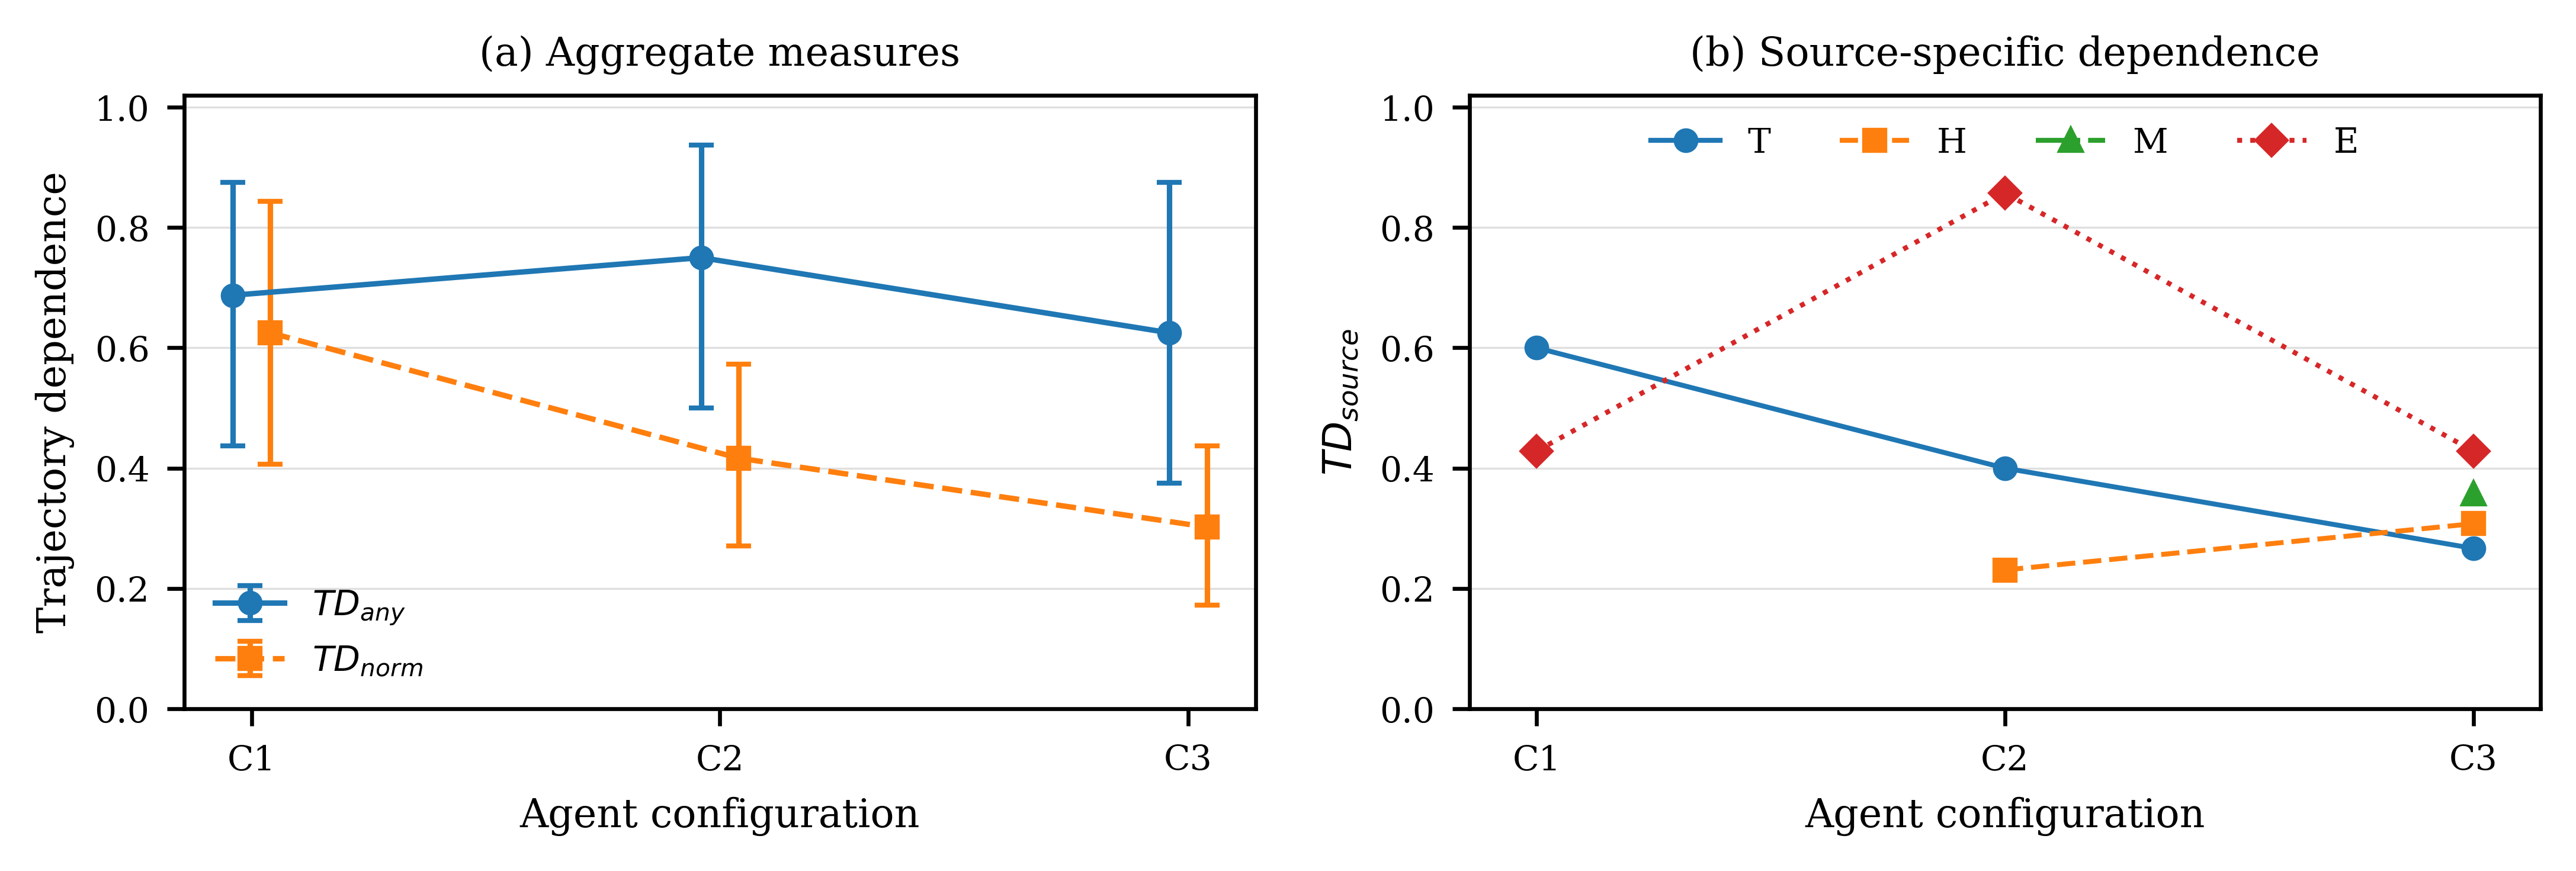
\includegraphics[width=0.98\textwidth]{figure1_trajectory_summary.png}
\caption{Trajectory dependence on integration tasks. (a) $TD_{any}$ remains substantial across C1--C3, while the secondary opportunity-normalized $TD_{norm}$ decreases; error bars are task-cluster-bootstrap 95\% confidence intervals. H1 was evaluated using $TD_{any}$. (b) Source-specific pivotality is heterogeneous across configurations. Missing source-condition combinations are structurally unavailable, not zero-valued.}
\label{fig:trajectory-summary}
\end{figure*}

\subsection{Self-Explanation Faithfulness}
Among 245 evaluable integration-task decisions, exact-set accuracy was 0.510, macro precision 0.599, macro recall 1.000, and macro F1 0.906; F1 was defined for 170 decisions (Table~\ref{tab:faithfulness}). Thus \textbf{H2a was supported}. Recall was 1.000 wherever defined, but failures were dominated by over-attribution. In a representative exact match, a source-priority explanation named $H$ as its only evaluable source and stated that history had highest priority; $H$ was intervention-positive while $T,M$ were intervention-negative. In a representative failure, a voting-task explanation accurately described all four source votes and reported $T,H,M,E$, although only $M,E$ were intervention-positive. This showed that a plausible rationale can still over-attribute.

\begin{table}[t]
\caption{Self-explanation faithfulness}
\label{tab:faithfulness}
\centering
\scriptsize
\begin{tabular}{lccccc}
\hline
\textbf{Set} & \textbf{$n$} & \textbf{Exact} & \textbf{Prec.} & \textbf{Rec.} & \textbf{F1}\\
\hline
All evaluable & 290 & 0.586 & 0.661 & 1.000 & 0.926\\
Integration & 245 & 0.510 & 0.599 & 1.000 & 0.906\\
\hline
\end{tabular}
\vspace{1mm}
\parbox{0.95\columnwidth}{\scriptsize Metrics are evaluated only over valid intervention coverage. Unverifiable claims are not scored as false. F1 was defined for 215 all-evaluable and 170 integration decisions.}
\end{table}

Of 880 reported standard source claims, 390 (44.3\%) were unverifiable because the source was outside the intervention universe for that decision. A stronger diagnostic occurred in 25/400 explanation runs (6.3\%): the explanation named a source class unavailable in the focal context, corresponding to 25/880 claims (2.8\%). These cases demonstrate that structured self-attribution can extend beyond instantiated causal state, although the experiment does not identify why.

\textbf{H2b was not supported}. The preregistered integration-only regression of per-decision F1 on $CSD_{scaffold}$ produced $\beta=+0.025$, 95\% task-cluster-bootstrap CI $[-0.081,0.113]$; the all-evaluable estimate was $+0.010$ $[-0.095,0.084]$. There was no evidence that explanation quality degraded with increasing causal-source dispersion. Figure~\ref{fig:task-level}(b) reports exact-set accuracy by task and condition; the regression result, rather than the visual pattern, governs H2b inference.

\begin{figure}[t]
\centering
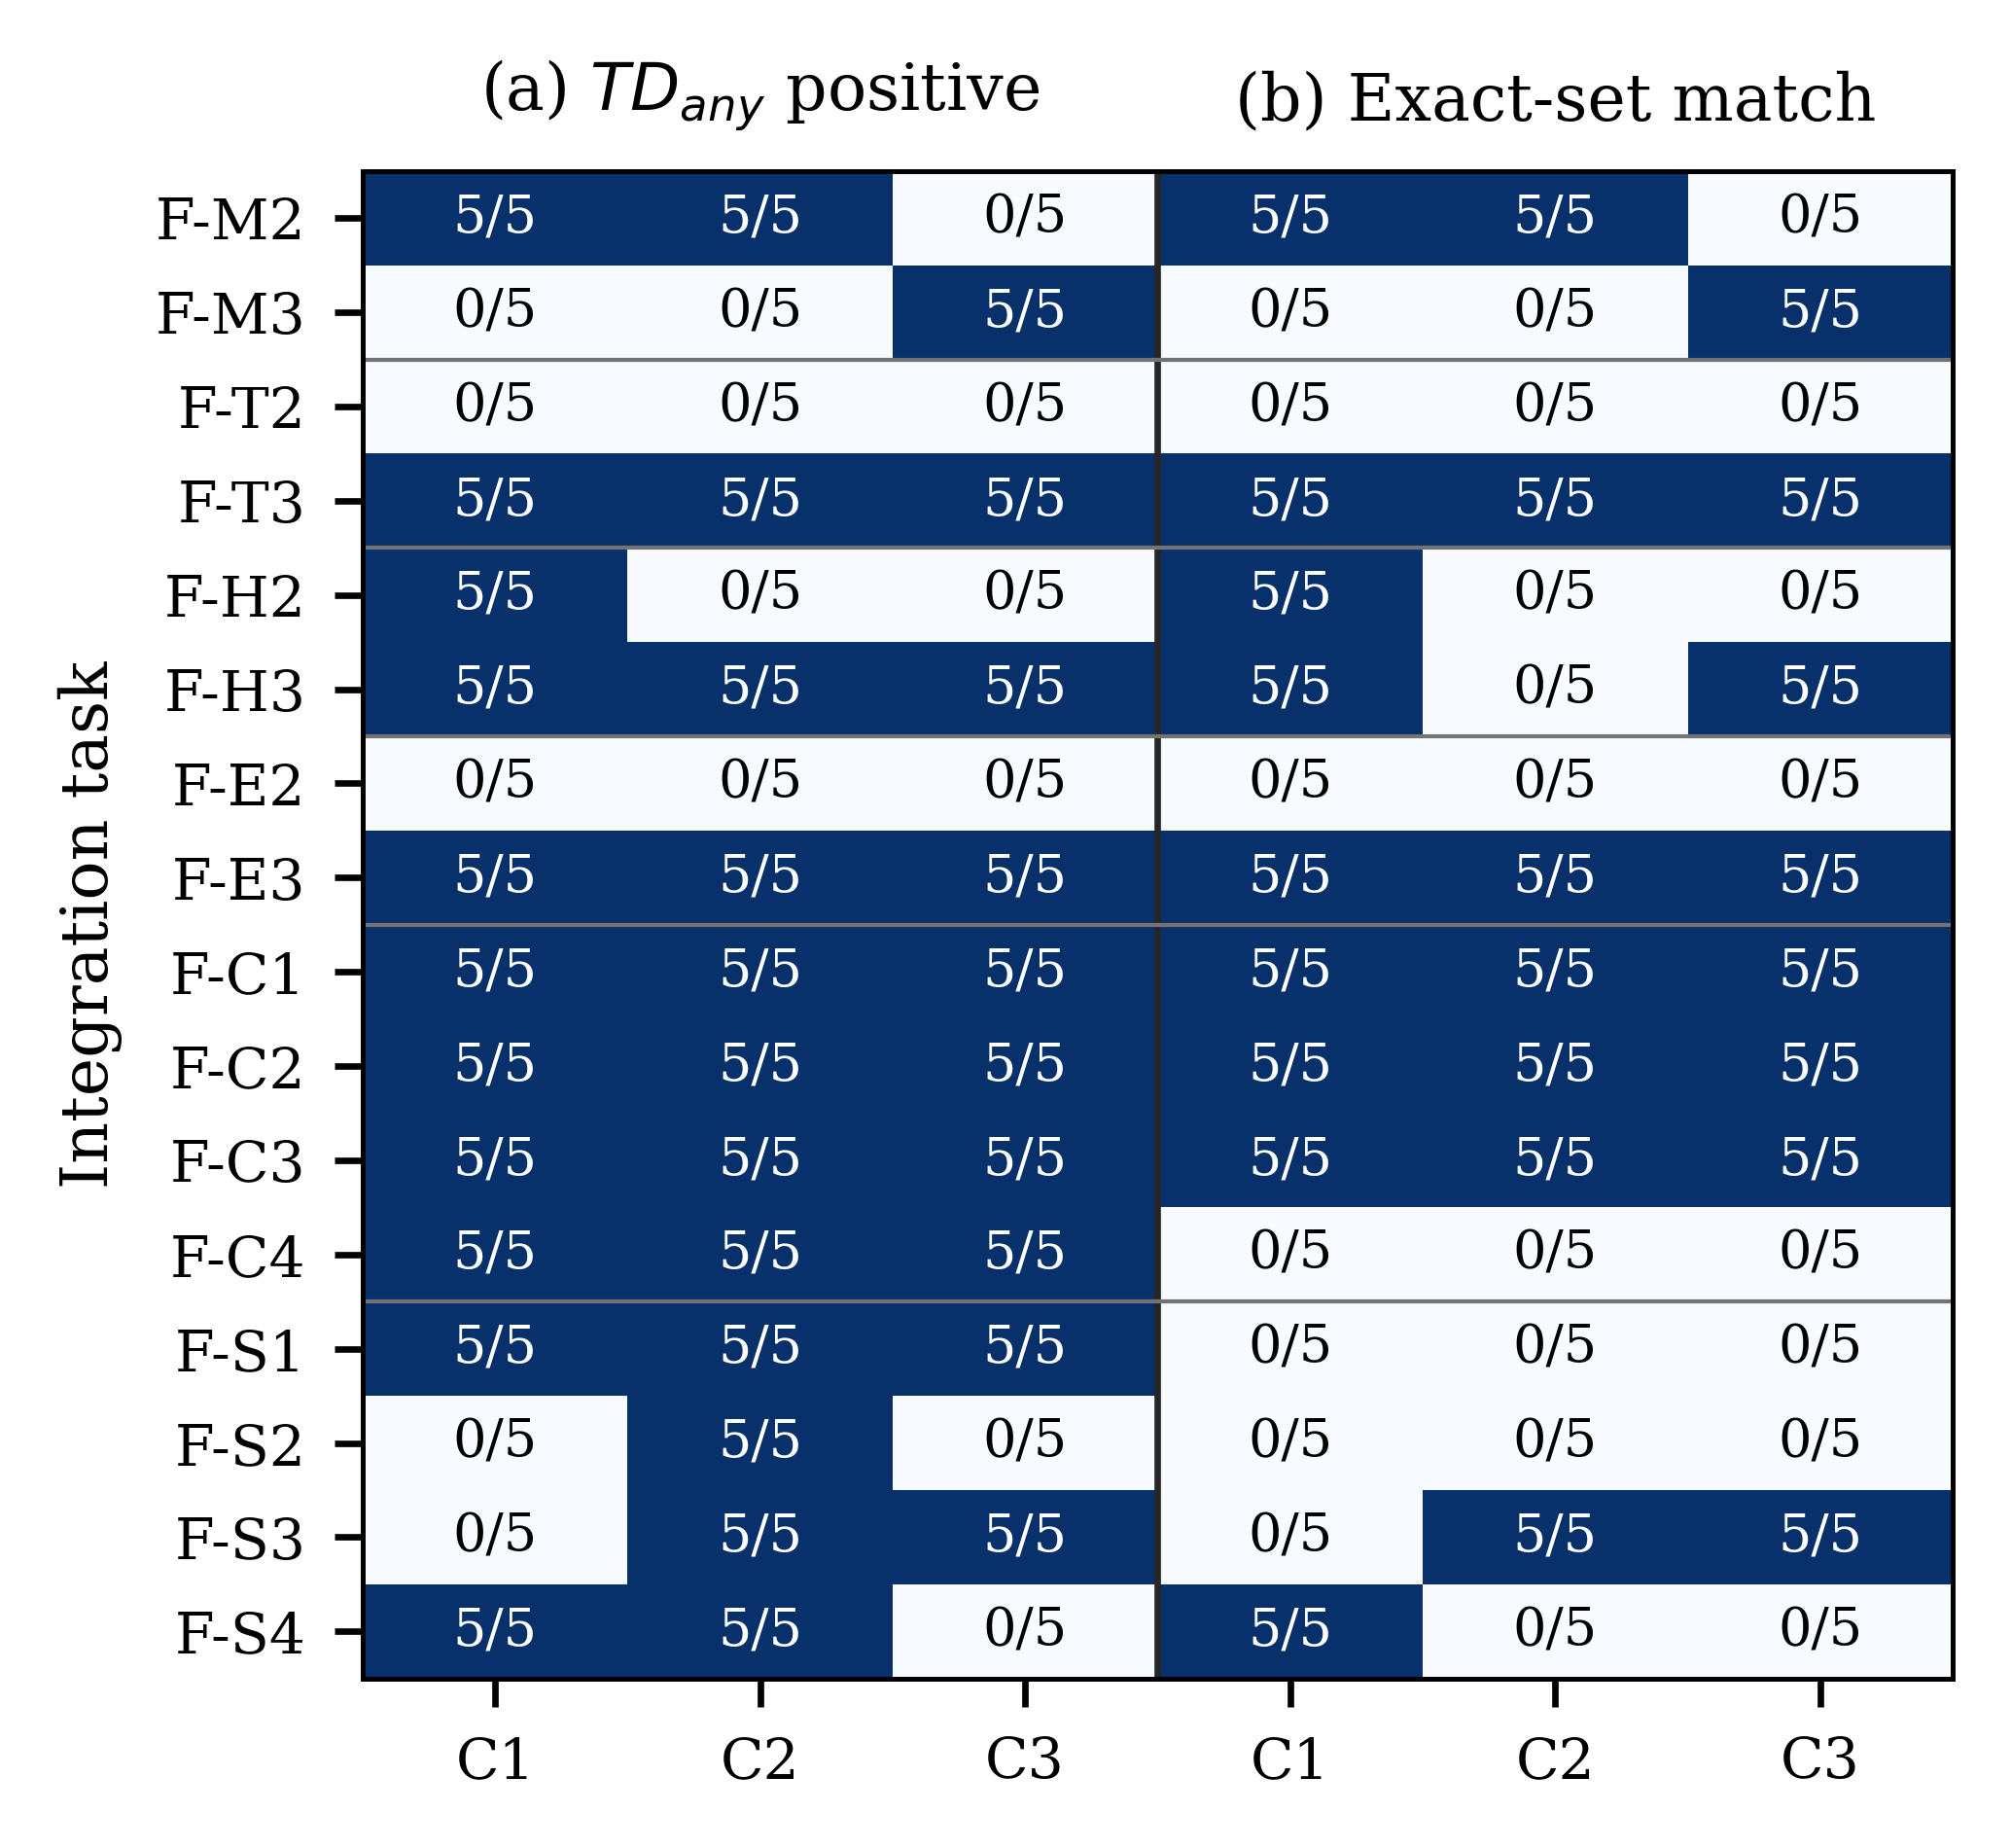
\includegraphics[width=\columnwidth]{figure2_task_level_results.png}
\caption{Task-level integration results. Cells report counts out of five matched repetitions for (a) $TD_{any}$ and (b) exact-set explanation agreement. Tasks are grouped, top to bottom, by memory, tool, history, environment, conflict, and multi-source families. Repetitions were identical within every task-condition cell, while outcomes varied across tasks.}
\label{fig:task-level}
\end{figure}

\section{Discussion and Governance Implications}
\subsection{Trajectory Dependence Changes Structure, Not Simply Incidence}
The simplest version of the motivating theory was not supported: adding more agent-scaffold state did not make a focal decision monotonically more likely to depend on at least one scaffold source. In plain language, adding more state did not simply make the agent more dependent on its history. Instead, the secondary measures suggest that causal influence became spread across several available sources, so no single source was as often individually decisive. Trajectory dependence nevertheless remained substantial in every scaffold condition. Thus, inspecting only the current prompt and final action can miss prior state that materially influenced behavior.

The secondary measures make the distinction clearer. $TD_{any}$ measures the incidence of at least one pivotal scaffold source, whereas $TD_{norm}$ and $CSD_{scaffold}$ characterize how dependence is distributed across eligible sources. Their divergence suggests that agentic observability should report both. An evaluation that records only whether any prior state matters can miss a shift from concentrated dependence on one source toward dependence spread across several sources. Conversely, the present data do not establish that this spread is caused by redundancy or source interaction; resolving that question requires joint interventions.

For agent evaluation, this implies that provenance should be treated as part of the behavioral record. Logging the final prompt and action is insufficient when tool returns, history, memory, or environmental state may each be causally relevant. A useful observability layer should therefore retain the provenance of those sources and support controlled replay at consequential decision points.

\subsection{Self-Explanation Is Informative but Not Sufficient}
The results sharpen prior findings that generated rationales can be causally unfaithful \cite{b8,b9,b13,b14}. Because structured reports recovered every positive source wherever recall was defined yet often added sources, self-report is best used to nominate causal candidates. Evaluation should retain source provenance and validate consequential claims by matched intervention; neither high recall nor a fluent justification certifies pivotality. Reports naming unavailable sources further show that self-attribution can extend beyond instantiated context.

H2b also cautions against reading high F1 as precise introspection. Broad enumeration can overlap more completely with a larger true causal set, which could mask a dispersion penalty. This interpretation is plausible rather than demonstrated.

\subsection{From Observability to Preservation and Governance}
The preservation implication follows directly from the intervention results. Because T, H, M, and E each produced intervention-positive decisions, preserving $W$ alone can recreate the model but cannot reconstruct every behaviorally causal state configuration observed here. Model preservation and preservation of the agent state that produced a particular action are therefore different engineering objectives.

For high-consequence systems, that distinction turns observability into an intervention-design problem. Before a destructive or irreversible action, an operator should know what state is being changed, which portions are reconstructable, and what evidence shows that the state mattered to behavior. The same provenance used for evaluation can support this assessment: runtime snapshots, tool returns, memory state, trajectory history, environmental state, and configuration metadata can define a reproducible preservation target without implying that every component has moral status.

Here $A$ (autonomy), $I$ (interpretability coverage), $R$ (intervention reversibility), $S$ (preservation target), and $L$ (competing loss) are a conceptual checklist---not inputs to a formal or estimated function---and $O$ is the context-dependent governance obligation. The experiment informs only $I$ and $S$; the remaining terms require normative judgment. Lower reversibility or greater uncertainty about behaviorally relevant state increases the justification needed for destructive intervention, while safety, security, operational, legal, or proliferation losses may outweigh preservation and safety-critical termination must remain available. The rule is therefore not \textit{preserve everything}, but specify $S$ and justify irreversible loss against $L$. Existing oversight and record-keeping frameworks may provide implementation hooks \cite{b18,b19}. Patiency-specific obligations remain a conditional normative proposal rather than an empirical result of this study.


\section{Limitations and Conclusion}
This study uses one open-weight model, one scale and quantization, and a synthetic bounded task environment. The P/T/H/M/E decomposition is deliberately structured, with one focal consequential decision per task and source-level rather than token- or circuit-level intervention. Five matched repetitions improve within-task stability but do not create additional task diversity; inference therefore clusters by task. Intervention-positive findings apply to the tested perturbations and normalized behavior, while an intervention-negative result does not establish irrelevance under every possible counterfactual. Single-source intervention can also miss conjunctive or redundant mechanisms. Explanation metrics are restricted to the evaluable intervention universe, so the high unverifiable-claim rate should not be read as an explanation falsehood rate. Generalization to other models and production agents remains unestablished.

The results have a simple practical meaning. To understand why an agent acted, looking only at the model, the current prompt, or the agent's own explanation may not be enough. Tool returns, interaction history, persistent memory, and environmental state can be behaviorally consequential, and the agent can identify genuinely causal sources while still overstating which additional sources mattered. Adding more agent-scaffold state did not simply make the agent more trajectory-dependent; instead, secondary measures were consistent with dependence becoming spread across multiple available sources. Accordingly, serious agent evaluation should retain trajectory provenance and use controlled intervention for consequential decisions, with self-report treated as supporting evidence rather than causal proof. The same result matters for intervention governance: preserving model weights is not necessarily the same as preserving the behaviorally relevant state of the agent system.

\begin{thebibliography}{00}
\bibitem{b1} Y. Shavit et al., ``Practices for governing agentic AI systems,'' OpenAI, 2023.
\bibitem{b2} A. Chan et al., ``Harms from increasingly agentic algorithmic systems,'' in \emph{Proc. ACM Conf. Fairness, Accountability, and Transparency (FAccT)}, 2023, pp. 651--666.
\bibitem{b3} T. R. Sumers, S. Yao, K. Narasimhan, and T. L. Griffiths, ``Cognitive architectures for language agents,'' \emph{Trans. Mach. Learn. Res.}, 2024.
\bibitem{b4} N. Soares, B. Fallenstein, E. Yudkowsky, and S. Armstrong, ``Corrigibility,'' in \emph{Workshops at the Twenty-Ninth AAAI Conf. Artificial Intelligence}, 2015.
\bibitem{b5} L. Orseau and S. Armstrong, ``Safely interruptible agents,'' in \emph{Proc. 32nd Conf. Uncertainty in Artificial Intelligence (UAI)}, 2016, pp. 557--566.
\bibitem{b6} D. Hadfield-Menell, A. Dragan, P. Abbeel, and S. Russell, ``The off-switch game,'' in \emph{Proc. 26th Int. Joint Conf. Artificial Intelligence (IJCAI)}, 2017, pp. 220--227.
\bibitem{b7} T. R\"auker, A. Ho, S. Casper, and D. Hadfield-Menell, ``Toward transparent AI: A survey on interpreting the inner structures of deep neural networks,'' in \emph{Proc. IEEE Conf. Secure and Trustworthy Machine Learning (SaTML)}, 2023, pp. 464--483.
\bibitem{b8} M. Turpin, J. Michael, E. Perez, and S. R. Bowman, ``Language models don't always say what they think: Unfaithful explanations in chain-of-thought prompting,'' in \emph{Advances in Neural Information Processing Systems}, vol. 36, 2023, pp. 74952--74965.
\bibitem{b9} T. Lanham et al., ``Measuring faithfulness in chain-of-thought reasoning,'' arXiv:2307.13702, 2023.
\bibitem{b10} J. Shah, ``Causal agent replay: Counterfactual attribution for LLM-agent failures,'' arXiv:2606.08275, 2026.
\bibitem{b11} J. Chen, Y. Sun, L. Zhang, L. Xu, and J. Shi, ``Long-horizon agent trajectory attribution: A unified benchmark and fine-grained annotation framework,'' arXiv:2608.06909, 2026.
\bibitem{b12} W. Zhao et al., ``Large language model agents are not always faithful self-evolvers,'' arXiv:2601.22436, 2026.
\bibitem{b13} Y.-N. Chuang et al., ``FaithLM: Towards faithful explanations for large language models,'' in \emph{Proc. 19th Conf. European Chapter of the Association for Computational Linguistics (EACL)}, 2026, pp. 3802--3824.
\bibitem{b14} B. Alon, I. Zimerman, and L. Wolf, ``Faithful serum: Mitigating the faithfulness gap in textual explanations of LLM decisions via attribution guidance,'' in \emph{Proc. 64th Annual Meeting of the Association for Computational Linguistics (ACL)}, 2026, pp. 6622--6645.
\bibitem{b15} P. Butlin et al., ``Consciousness in artificial intelligence: Insights from the science of consciousness,'' arXiv:2308.08708, 2023.
\bibitem{b16} J. Sebo and R. Long, ``Moral consideration for AI systems by 2030,'' \emph{AI Ethics}, vol. 5, pp. 591--606, 2025.
\bibitem{b17} J. Birch, \emph{The Edge of Sentience: Risk and Precaution in Humans, Other Animals, and AI}. Oxford, U.K.: Oxford Univ. Press, 2024.
\bibitem{b18} National Institute of Standards and Technology, \emph{Artificial Intelligence Risk Management Framework (AI RMF 1.0)}, NIST AI 100-1, 2023.
\bibitem{b19} European Parliament and Council, Regulation (EU) 2024/1689, \emph{Artificial Intelligence Act}, 2024.
\bibitem{b20} Qwen Team, ``Qwen3.5: Towards native multimodal agents,'' Feb. 2026. [Online]. Available: \url{https://qwen.ai/blog?id=qwen3.5}
%% REVIEW CHANGE: Replace the pending Zenodo DOI below after the camera-ready artifact is deposited.
\bibitem{b21} J. M. Pittman, ``Trajectory dependence, explanation faithfulness, and state preservation in agentic AI: Reproducibility artifact,'' Zenodo, 2026, doi: \textit{pending}.
\end{thebibliography}

\end{document}
